Os conjuntos que representam os conceitos são organizados em  módulos. Isso ocorre porque muitos conceitos apresentam similariedades, sendo razoavel conceber uma taxonomia desses conjuntos organizando-os em conjuntos maiores. A figura \ref{module} apresenta a estrutura de módulos (a fim de evitar poluição visual, as relações serão apresentadas em outra figura). 

\begin{figure}[H]
  \centering
  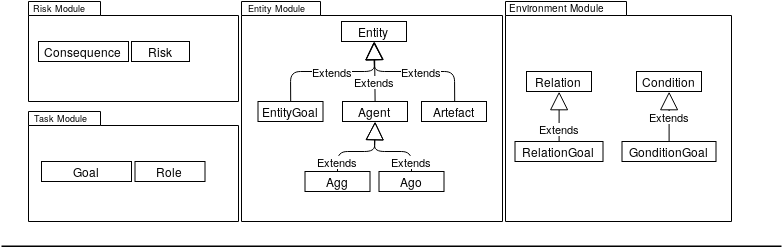
\includegraphics[width=1\linewidth]{figure/Module.png} 
  \caption{A estrutura geral das classes do modelo}
  \label{module}
\end{figure}

Assim sendo, assumindo que existe $\Omega_{Model}$ (um conjunto global onde todos os outros conjuntos do modelo estão contidos nele), os módulos são representados da seguinte maneira; 

\begin{equation} 
    \Omega_{Model} = \{ M_{Risk}, M_{Task}, M_{Entity}, M_{Environment}\}
\end{equation}
\label{modules}


O mundo sobre o qual este modelo pretende representar trabalha com o fato de que tanto agentes bem como artefatos possuem algumas propriedades em comum, que é; existem, ocupam lugar no espaço, estão sujeitos ao tempo, apresentam estados e participam de processos. Essa premissa possue os seus fundamentos alicerçados em \ref{agent} e \ref{artefact} e isso será demonstrado com maior rigor no texto que se segue. Tendo em vista o ocorrência de certos conceitos necessários para lidar com essas questões, se fez necessário definir um módulo de entidades para agrupa-los em uma estrutura única. Esse módulo é composto pelos seguintes conceitos;

\begin{equation} 
M_{Entity} = \{ Entity, Agent, Artefact, EntityGoal, Agg, Ago\}
\end{equation}\label{modent}

\textbf{Entity} - O termo entidade é sujeito a profundos debates filosóficos, porém neste texto o termo é usado para referenciar uma "coisa" que pode ser identificada, como uma pessoa, companhia ou um evento \cite{entity}. É dado que as propriedades anteriormente mencionadas caracterizam as "coisas" que podem ser identificadas, logo entidades. É digno de nota a existência de entidades que não se adequam a todas essas propriedades. Contudo, essas propriedades fazem referência ao que se caracteriza por entidade respeitando o conceito padrão \cite{entity} e restringindo para o escopo deste modelo. Isso contempla tanto os agentes assim como artefatos, como fica claro na relação \ref{defineentity}. O texto a seguir demonstra como essas propriedades se aplicam a agentes e a artefatos (se isso ficar demonstrado, logo fica demonstrado que são entidades).

\textit{Existe -} Dado como quantificador, se há um ou mais, então existe. Assim sendo, tanto agentes como artefatos existem porque, dentro da representação, ambos fazem referência a coisa que correspondem a um ou mais. 

\textit{Ocupa lugar no espaço, estão sujeitos ao tempo - } Como definido em \ref{agent} e \ref{artefact}, ambos são situados em ambientes. 
Isso possibilita inferir que se faz necessário a presença de um conceito que se apresente como uma propriedade de estado para agentes e artefatos. Um ambiente, no contexto onde os agentes e artefatos são usados para representar atividades das pessoas, condiz com a relação de espaço e tempo. 

\textit{Participa de Processos -} Processos podem constituir entidades bem como entidades necessariamente constituem processos por intermédio a ação que aquelas manifestam nesses. No que se verifica ao primeiro caso, é possível usar o ser humano como exemplo - onde
a entidade humano é formulada por uma série de processos bio-químicos. Sobre o segundo caso, relações climáticas exemplificam isso, onde a água é uma entidade presente em processos termodinâmicos. 

\textit{Apresenta estados -} O fato de que artefatos bem como agentes apresentam atributos (que podem mudar e podem assumir diferentes valores no que tange aos eventos externos e internos), então ambos também apresentam a concepção de estados (sendo esse termo usado diretamente em certos pontos dos textos presentes tanto em \ref{agent} \ref{artefact}). 


\begin{equation} \label{defineentity} 
( Agent \cup Artefact ) \subset Entity
\end{equation}

\textbf{Agent} - Esse estudo adota a definição de agentes presentes no primeiro parágrafo da seção \ref{agent}. Isso implica entidades autônomas, ou seja -que apresenta a capacidade de agir por si mesma quando diante de condições onde isso é necessário. A seção \ref{agent}, apresenta o conceito de agentes inteligentes e esse mesmo conceito é adotado neste modelo. 

Não é preocupação deste estudo delimitar as representações do agente bem como definir algoritmos para verificar como se da as relações de tomada de decisão. Assim sendo, fica em aberto para o modelador definir como se dá os processos de tomada de decisão, estados internos e modelos de representação que serão usados para definir o comportando do agente. 

\textbf{Artefact} - são entidade que existem para que os agentes possam cumprir com os seus objetivos e que apresentam interface de uso, instruções de operação, funcionalidade e estrutura-comportamento. Essas entidades não são orientados a objetivos e 
não apresentam capacidade de comunicação como definido na seção \ref{artefact}. Predicados que contemplam esses aspectos do artefato serão apresentados mais adiante ao decorrer do texto. 

Os agentes são autônomos e orientados a objetivos sendo esses dois elementos descaracterizantes do que se defini como por artefato. Logo, apesar de agentes e artefatos serem entidades, não é possível existir um agente que seja artefato ou um artefato que seja agente, o que é dado por \ref{agentsartefactvoid}. 

\begin{equation} \label{agentsartefactvoid}
    Agent \cap Artefact = \{ \emptyset \}
\end{equation}


\textbf{EntityGoal} - Condiz a subconjuntos de \textbf{Entity} que, por intermédio de um predicado que será apresentado posteriormente, se relacionam com elementos do conjunto \textbf{Goal} (representam os objetivos). Assim sendo, consiste nas entidades necessárias que devem estar presentes no ato da execução de um certo objetivo para que este possa ser alcançado. Para exemplificar é possível conceber o seguinte cenário; 

\textbf{Exemplo da Redação:} "O Professor Aristóteles definiu uma atividade; Escrever uma redação sobre o livro Metafísica. Para isso, o aluno Alexandre o Grande deve escrever um dado texto, deve ler o livro sobre o tópico em definido, deve pegar uma folha, deve pegar um lápis e escrever a redação".  


Neste modelo, esse cenário pode ser especificado da seguinte forma; $E = \{aristoteles, alexadre, folha, lapis, livro\}$, em termos de objetivo (esse conceito será descrito com maior detalhe no texto em diante) há três $G = \{ g_0, g_1,g_2\}$  onde $g_0$ corresponde ao ato do professor definir a atividade, $g_1$ corresponde ao ato de ler o livro e $g_2$ ao ato de escrever a redação. Então, é possível 
definir três subconjuntos de $E$, esses são os conjuntos \textbf{EntityGoal}, $E_g = \{ eg_{0}, eg_{1}, eg_{2} \}$, onde $eg_{0} = \{ aristoteles \}$ $eg_{1} = \{ alexandre, livro\}$ e $eg_{2} = \{ aluno, folha, lapis \}$. Em termos de relação, que será melhor trabalhado 
em partes futuras deste texto, considera-se que $eg_0$ se relaciona com $g_0$, $eg_1$ se relaciona com $g_1$ e $eg_2$ com $g_2$.

\textbf{Agg, Ago} - ambos correspondem ao conjunto de agentes que atingiram um determinado objetivo. Contudo, \textbf{Agg} faz referência aos gentes que atingiram o objetivo sem serem obrigados a isso, e \textbf{Ago} condiz aos agentes que atingiram o objetivo sendo obrigados a isso. Em um primeiro momento essa diferença para ser desnecessária, mas é relevante para criação de regras que serão apresentadas futuramente. A necessidade deste conjunto pode por ser demonstrada com o \textbf{Exemplo da Redação}, pois Alexandre e Aristóteles são obrigados a alcançar os objetivos. Então, é definido por $Ago = \{ ago_0, ago_1, ago_1 \}$ onde $ago_0 = \{ \emptyset \}$ , $ago_1 = \{ \emptyset \}$ e $ago_2 = \{ \emptyset \}$. Ao atingir $g_0$ o $ago_o = \{ artistoteles\}$ pois o professor cumpriu com o objetivo de passar a atividade. O mesmo ocorre para $ag_1$, $g_1$ e para $ag_2$, $g_2$.


\textbf{O Módulo de Atividades} - \textit{Task Module} representado por $M_{Task}$ condiz com os conceitos relacionados aos obetivos que devem ser atingidos bem como aos papéis que são assumidos pelos agentes.
\begin{equation}
    M_{Task} = \{ Goal, GoalPreRequisite, Role \}
\end{equation}

\textbf{Goal} - faz referência aos objetivos que devem ser atingidos pelos agentes. Os fundamentos semânticos deste conjunto está presente na seção \ref{sma} mais especificamente na subseção \ref{moiseformalizesma}. Neste modelo, um objetivo é descrito em termos de $eg$ e $rg$ (conjuntos de relacionamentos, será explicado com maior detalhes no texto adiante), que são as entidades e os relacionamentos (será explicado) que devem ser ser feitos para que o objetivo possa ser dado como concluído. Com o propósito de explorar com maior granularidade as relações entre o agente e o objetivo, neste modelo o conceito de missão foi removido. Como será apresentado posteriormente, as relações deônticas entre os papéis se dão com o objetivo e não com a missão. O estudo presente no \textit{MOISE+} faz uso de grafos para representar objetivos-subobjetivos. Esse modelo não importou a estrutura em grafos para descrever o comportamento de objetivos. 

\textbf{Role} - apresenta o papel que um agente pode adotar dentro de um \textit{SMA}. Esse conceito também é importado no \textit{MOISE+} 
\ref{moiseformalizesma} e define as relações deonticas entre os agentes e os objetivos. Para exemplificar, pode-se considerar o \textbf{Exemplo da Redação} onde existe dois agentes $Agent = \{ aristoteles, alexandre \}$, existe dois papéis $Role = \{ professor, aluno\}$. Neste caso, o agente $aristoteles$ é o $professor$ e o agente $alexandre$ é o $aluno$.

\textbf{O Módulo de Ambiente} - \textit{Environment Module} - consiste em conjuntos que representam relações e condições ambientes, esses são;

\begin{equation}
    M_{Environment} = \{ Relation, Condition, Circumstance, ReationGoal, ConditionGoal \}
\end{equation}

\textbf{Relation} - Uma entidade estabelece relações com outras entidades ao seu redor \cite{entity}. No modelo proposto neste texto, 
os pesquisadores optaram por definir um conjunto que representa essas relações. Os pesquisadores optaram por um conjunto para representar
os relacionamentos entre as entidades porque isso possibilita identifica-los. Isso facilita o desenvolvimento de raciocínios. O uso 
dos relacionamentos podem ser exemplificado por meio do \textbf{Exemplo da Redação}. Ao definir uma atividade, o professor Aristóteles
, que é uma entidade, estabeleceu uma relação com o seu aluno Alexandre, representado aqui por $relAristotelesAlexandre$. Para cumprir com essa tarefa o aluno teve de ler o livro - $relAlexandreLivro$, teve de pegar uma folha - $relAlexandreFolha$, teve de pegar um lápis $relAlexandreLapis$ e teve de escrever a redação o que implica em uma relação entre lápis e folha $relLapisFolha$. Portanto, o conjunto de relacionamentos se dá da seguinte maneira;

\begin{eqnarray}\label{Environment}\nonumber
    M_{Environment} = \{ relAristotelesAlexandre, relAlexandreFolha, relAlexandreLivro, \\ \nonumber
     relAlexandreLapis, relLapisFolha \}
\end{eqnarray}

Obviamente, cada entidade do grupo \textit{Relation} tem uma vínculo com elementos do grupo \textit{Entity}, como por exemplo $relAlexandreFolha$ apresenta um dado vinculo com as entidades $Alexandre$ e $Folha$. Há um predicado que trata disto e será exibido posteriormente. Assim como o conjunto $EntityGoal$, existe relacionamentos que devem estar presentes para que dados objetivos possam ser atingidos, revelando - portanto - a necessidade de um conjunto para representar esse tipo de situação, que neste caso é $RelationGoal$. O exemplo em análise é descrito por três objetivos. O objetivo $g_0$ corresponde ao ato  do professor definir a atividade. Esse objetivo não pode ser cumprido sem relacionamento $relAristotelesAlexandre$. Portanto, existe $rg_0$ associado a $g_0$ onde $rg_0 = \{ relAristotelesAlexandre \}$ e que $rg_0 \subset RelationGoal$. O conjunto $g_1$ está relacionado com $rg_1$ e esse, por sua vez, é composto por $\{ relAlexandreFolha\}$. O conjunto $g_2$ está relacionado com $rg_2$ e os elementos correspondem a $\{ relAlexandreLapis, relLapisFolha, relAlexandreFolha\}$.

\textbf{Condition} - Esse conjunto representa as condições que devem ser mantidas para que um dado objetivo possa ser alcançado. Em analogia a $EntityGoal$ e a $RelationGoal$, há um conjunto denominado de $ConditionGoal$ que define essas condições para os objetivos. Para exemplificar o uso deste conjunto é possível considerar o \textbf{Exemplo da Redação}. Com certeza nenhum dos três objetivos se tornam viáveis se não houver luz suficiente para que todos possam ver. O ambiente deve ser mantido em um certo silêncio, do contrário não há possibilidade do professor e do aluno exercer suas atividades intelectuais. Assim sendo é possível definir duas entidades; $Condition = \{ luz,silencio \}$. Ambas as condições são válidas para todos os objetivos (para esse
exemplo), portanto existe um $cg_1 = \{ luz,silencio \} | CondtionGoal = \{ cg_1 \}$, sendo que $cg_1$ estabelece relações com 
$g_0$, $g_1$ e $g_2$.

Certos relacionamentos, que serão apresentados com maior riqueza de detalhes mais adiante, exigem definir uma certa abstração entre \textbf{Condition} e \textbf{Relation}. Assim sendo, os pesquisadores assumem a existência de um conjunto \textbf{Circumstance} que é dado pela seguinte relação; 

\begin{equation}
    Circumstance = \{ Relation, Condition \} |  Relation \cap Condition = \{ \emptyset \}
\end{equation}


\textbf{Módulo de Risco} - \textit{Risk Module} contem conjuntos que correspondem a conceitos relacionados a temática da segurança.
O módulo de risco é dado pela relação que se segue;

\begin{equation}
    M_{Risk} = \{ Risk, Consequence \}
\end{equation}

\textbf{Risk} - Na seção \ref{risksec} o termo risco é usado para referenciar a um evento que apresenta um potencial de ocorrer e que gera consequências negativas as pessoas associadas quando acontece. Para exemplificar pode-se considerar uma condição onde um eletricista está trocando um disjuntor de um quadro elétrico. Nesse processo, o eletricista está sujeito ao risco de ser eletrocutado. Essas consequências negativas também são representadas por um conjunto, e esse é \textbf{Consequence}. O uso deste conjunto pode ser apresentado utilizando esse mesmo exemplo do eletricista, pois a consequência de se submeter a um evento desses implica morte (nem sempre é assim, mas para efeitos didáticos pode-se considerar que o quadro elétrico é de certa potência que a morte é certa para o profissional que for eletrocutado).